\documentclass{article}
\usepackage{etoolbox}
\usepackage{graphicx}

\ifdef{\myoutput}{}{\def\myoutput{concept}}
\ifdef{\myversion}{}{\def\myversion{1}}

\usepackage[output=\myoutput
,numberofversions=4
,version=\myversion
,seed=4
,randomizequestions=true
,randomizeanswers=true
,writeRfile=true
]{mcexam}

\usepackage[margin=0.95in]{geometry}
\usepackage{multicol}

\usepackage{fancyhdr,lastpage}
\pagestyle{fancy}
\fancyhf{}
\renewcommand{\headrulewidth}{1pt} 
\renewcommand{\footrulewidth}{1pt}
\lfoot{\mctheversion}
\rfoot{Page \thepage\ of \pageref{LastPage}}
\lhead{Quiz 4.1 \& 4.2 Version \fbox{\myversion} \\ MAT 2000: Introduction to Statistics}
\rhead{Name Print): \hspace{2.5 in}}

\usepackage{calc}
\renewenvironment{setmcquestion}
{\begin{minipage}[t]{\linewidth-\labelwidth}}
	{\end{minipage}\par}
	
\renewenvironment{setmcquestioninstruction}
{\begin{minipage}{\textwidth}}
	{\end{minipage}}
	
\renewenvironment{setmcanswers}{}{}
\setlist[setmcquestions]{label=\mcquestionlabelfmt{*}.
	,ref=\mcquestionlabelfmt{*}
	,itemsep=0.5\baselineskip
	,topsep=1\baselineskip
}

\renewcommand\mcversionlabelfmt[1]{\arabic{#1}}

%copy-pasting from MS Word, use regex to find [\*]*[a-d]\. and replace with \answer 

\raggedbottom

\begin{document}
	Circle the correct answer for each question.  If you're unsure, you can write numbers 1, 2, 3, etc. next to the choices to get partial credit.\\[.5cm]
	\begin{mcquestions}
		\question Suppose a confidence interval is constructed using repeated tests of significance to develop an interval of plausible values.  Two-sided tests are used each time with the following null hypotheses and resulting p-values.
		\begin{center}
			\begin{tabular}{llp{.75in}ll}
				Null              & p-value & & Null              & p-value  \\
				$\pi = 0.45$ & 0.009   &                                 & $\pi = 0.53$ & 0.787    \\
				$\pi = 0.46$ & 0.032   &                                 & $\pi = 0.54$ & 0.572    \\
				$\pi = 0.47$ & 0.062   &                                 & $\pi = 0.55$ & 0.373    \\
				$\pi = 0.48$ & 0.126   &                                 & $\pi = 0.56$ & 0.142    \\
				$\pi = 0.49$ & 0.371   &                                 & $\pi = 0.57$ & 0.077    \\
				$\pi = 0.50$ & 0.598   &                                 & $\pi = 0.58$ & 0.042    \\
				$\pi = 0.51$ & 0.733   &                                 & $\pi = 0.59$ & 0.021    \\
				$\pi = 0.52$ & 0.986   &                                 & $\pi = 0.60$ & 0.003   
			\end{tabular}
		\end{center}
		Using the results, give a 95\% confidence interval.
		\begin{mcanswerslist}
			\answer (0.50, 0.54)
			\answer[correct] (0.47, 0.57)
			\answer (0.45, 0.60)
			\answer (0.46, 0.58)
		\end{mcanswerslist}
		
		\question Commercial fisherman working certain parts of the Atlantic Ocean sometimes find efforts being hindered by the presence of whales. Ideally, the whales could be scared away without frightening the fish. Experience has shown that whales leave the sight of a fishing boat 40\% of the time. One of the strategies being experimented with is to transmit underwater sounds of a killer whale. On the 52 occasions that this technique has been tried, the technique worked 24 times (that is, the whales immediately left the area).
		A 99\% confidence interval for $\pi$ is $(0.29, 0.65)$. How would you interpret this interval?
		\begin{mcanswerslist}
			\answer When underwater sounds of killer whales are transmitted, fishermen can be are 99\% confident that whales leave the sight of a fishing boat 46\% of the time.
			\answer[correct] When underwater sounds of killer whales are transmitted, fishermen can be 99\% confident that whales leave the sight of a fishing boat between 29\% and 65\% of the time.
			\answer 99\% of whales will leave the sight of a fishing boat if the whales hear sounds of a killer whale.
			\answer If another sample of 52 occasions is collected, a 99\% chance exists that the sample proportion of whales who leave the sight of a fishing boat will be between 0.29 and 0.65.
		\end{mcanswerslist}
		
		\question Let $\pi$ be some population proportion of interest and suppose a 99\% confidence interval for $\pi$ is calculated to be (0.32, 0.41) and a 95\% confidence interval is calculated to be (0.34, 0.39). Also, suppose the hypothesis test is $H_0: \pi = 0.33$ and $H_A: \pi \neq 0.33$. What can be said about the corresponding p-value for this test?
		\begin{mcanswerslist}
			\answer The corresponding p-value will be less than 0.01.
			\answer[correct] The corresponding p-value will be between 0.01 and 0.05.
			\answer The corresponding p-value will be between 0.05 and 0.10.
			\answer The corresponding p-value will be greater than 0.10.
		\end{mcanswerslist}
		
		\question Suppose a test of significance is conducted with $H_0: \pi = 0.50$ and $H_A: \pi \neq 0.50$ with a resulting p-value of 0.07.  Also, 99\% and 95\% confidence intervals are constructed from the data.
		What will be true about the confidence intervals?
		\begin{mcanswerslist}
			\answer[correct] Both the 99\% and the 95\% intervals will contain 0.50.
			\answer Neither the 99\% nor the 95\% intervals will contain 0.50.
			\answer The 99\% interval will contain 0.50, but the 95\% interval will not contain 0.50.
			\answer The 99\% interval will not contain 0.50, but the 95\% interval will contain 0.50.
		\end{mcanswerslist}
		
		\question A 95\% confidence interval for a population proportion is (0.67, 0.83).\\
		
		What is the sample proportion?
		\begin{mcanswerslist}
			\answer 0.67
			\answer 0.83
			\answer[correct] 0.75
			\answer 0.08
		\end{mcanswerslist}
		
		\question[follow] What is the margin of error from the question above?
		\begin{mcanswerslist}
			\answer 0.67
			\answer 0.83
			\answer 0.75
			\answer[correct] 0.08
		\end{mcanswerslist}
		
		
		\question A 99\% confidence interval for a population proportion is $0.20 \pm 0.09$. What is the confidence interval?
		\begin{mcanswerslist}
			\answer (0.155,0.245)
			\answer (0.21,0.22)
			\answer[correct] (0.11,0.29)
			\answer The confidence interval cannot be determined.
		\end{mcanswerslist}
		
		\question The spinning dancer (or silhouette illusion) is a moving image of a woman that appears to be spinning.  Some people see her spinning clockwise and some see her spinning counterclockwise.  A student showed other students this and found that 30 out of 50 (or 60\%) saw her spinning clockwise.  The student researcher was interested in the probability of a randomly chosen student that would see the dancer spinning clockwise.  The student created the following null distribution.
		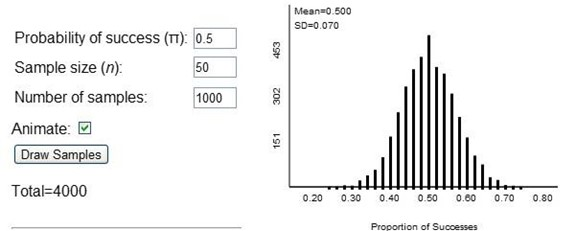
\includegraphics[width=\textwidth]{null_dancer.jpg}
		Using the information provided above, determine a 2SD confidence interval for the long-run probability a randomly chosen student would see the woman spinning clockwise.  (Don't use any other applet to do this, just the information above.)
		\begin{mcanswerslist}
			\answer (0.36, 0.64)
			\answer[correct] (0.46, 0.74)
			\answer (0.53, 0.67)
			\answer (0.43, 0.57)
		\end{mcanswerslist}
		
		\question Many studies have investigated the question of whether people tend to think of an odd number when asked to think of a single-digit number (0 through 9; 0 is considered an even number). When asked to pick a number between 0 and 9, out of 70 students, 42 chose an odd number. Let the parameter of interest, $\pi$ , represent the probability that a student will choose an odd number.\\
		Are conditions met to use theory-based methods for conducting a 95\% confidence interval?
		\begin{mcanswerslist}
			\answer Yes, because there were two possible outcomes.
			\answer Yes, since the number of students is larger than 30.
			\answer[correct] Yes, since the number of students who chose an odd number, and the number of students who chose an even number, are both greater than 10.
			\answer No, since the sample size is too small.
		\end{mcanswerslist}
		
		\question Hill and Barton (Nature, 2005) conducted a study to investigate whether Olympic athletes in certain uniform colors have an advantage over their competitors. They noted that competitors in the combat sports of boxing, tae kwon do, Greco-Roman wrestling, and freestyle wrestling are randomly assigned to wear red or blue uniforms.  For each match in the 2004 Olympics, the uniform color of the winner was recorded. Hill and Barton found that in the 457 matches, the competitor wearing red won 248 times (54.3\%), whereas the person wearing blue won 209 times (45.7\%).\\
		Based on these data, use the 2SD method to construct a 95\% confidence interval for the proportion of matches won by competitors wearing red uniforms.
		\begin{mcanswerslist}
			\answer[correct] (0.497, 0.589)
			\answer (0.454, 0.546)
			\answer (0.493, 0.593)
			\answer (0.483, 0.602)
		\end{mcanswerslist}
		
		\question Suppose a 95\% confidence interval for a population proportion is (0.21, 0.43). How would the width of the confidence interval change if the confidence level was changed?
		\begin{mcanswerslist}
			\answer Both a 99\% confidence interval and a 90\% confidence interval would both be wider.
			\answer[correct] A 99\% confidence interval would be wider and a 90\% confidence interval would be narrower.
			\answer A 99\% confidence interval would be narrower and a 90\% confidence interval would be wider.
			\answer Both a 99\% confidence interval and a 90\% confidence interval would be narrower.
		\end{mcanswerslist}
		
		
	\end{mcquestions}
\end{document}